%%%%%%%%%%%%%%%%%%%%%%%%%%%%%%%%%%%%%%%%%%%%%%%%%%%%%%%%%%%
%                                                         %
%                      Cliff Watkins                      %
%                                                         %
%             Draft of Mixed Layer Depth Paper            %
%                                                         %
%%%%%%%%%%%%%%%%%%%%%%%%%%%%%%%%%%%%%%%%%%%%%%%%%%%%%%%%%%%

\documentclass{article}

% Default Packages
\usepackage[utf8]{inputenc}
\usepackage[english]{babel}
\usepackage[affil-it]{authblk}
\usepackage{geometry}
 
% Graphics package
\usepackage{graphicx}
\graphicspath{ {images/} }

% Maths packages
\usepackage{amssymb}
\usepackage{amsmath}
\newtheorem{theorem}{Theorem}

\usepackage{setspace}


% Bibliography Packages
\usepackage{csquotes}
%\usepackage{biblatex}
\usepackage[backend=biber,style=ieee,sorting=ynt]{biblatex}
\addbibresource{MLD.bib}

\title{Storm to seasonal life cycles of the mixed layer depth across the Mid-Atlantic Bight from high-frequency radar remote sensing}

\author[1]{C E Watkins}
%\author[1]{John Wilkin}
%\author[2]{Daniel B Whitt}
%\author[1]{Scott Glenn}

\affil[1]{Department of Marine and Coastal Sciences, Rutgers, New Brunswick, NJ, USA}
%\affil[2]{National Center for Atmospheric Research, Boulder, CO, USA.}

%\date{April 2017}
 
\begin{document}
\pagenumbering{arabic}
\maketitle
 
\begin{abstract}
By developing and using a novel model for determining the mixed-layer depth using a combination of high-frequency (HF) radar and and model-derived 10-m winds, we show the shelf-wide behavior of the surface mixed layer depth (MLD) in response to both a tropical cyclone and seasonal forcing in the in the Mid-Atlantic Bight (MAB). 
By comparing the modeled MLDs to in-situ observations through the life cycle of Hurricane Irene (2011), we show that the storm-driven deepening can be quantified using a novel cost function to solve an inverse solution to Pollard and Millard’s (1970) slab model of inertial motion.
Using this, we map the rapid ahead-of-eye deepening of the mixed layer moving from Southern MAB northward toward New York City ahead of Hurricane Irene (2011) at the leading edge the wind field that entrained the cooler waters under the seasonal thermocline and consistent with the northward storm track.
Hurricane Irene also influenced the MLD in the Northern MAB, off Cape Cod, even though landfall occurred near New York City more rapidly due to multiple factors such as weaker initial stratification, storm track, and larger wind field extending seaward during extratropical transition.
This method allows for analysis of the spatial structure of the seasonal cycle in MLD, where the transition from highly stratified to a cooler single-layer system moves from South to North in response to the storm-forcing and diminishing solar intensity of Autumn.
\end{abstract}

\doublespacing
\section*{Introduction}
The coastal surface mixed layer depth (MLD) impacts air-sea interaction, ocean/bottom interaction, and biogeochemistry \cite{Kraus1967,ambler2013seasonal,chen2018seasonal}.
The uniform temperature, salinity, and density of the surface mixed layer dictates the oceanic response to surface stresses and mediates the biological capacity of the water column \cite{Carvalho2017}.
In the open ocean, this relatively homogeneous water mass is defined above by the air-sea interface and below by a change in temperature, salinity, or density that defines a mixed layer depth (MLD) \cite{Thomson2003,Jeronimo2010}.


The Mid-Atlantic Bight (MAB) is a geographic region of the continental shelf between Cape Hatteras in the South and the Gulf of Maine or the Nantucket Shoals in the North \cite{Houghton1982}.
For coastal oceans such as the Mid Atlantic Bight, the mixed layer behaves differently because the bottom boundary is within the nominal range of MLD for the global ocean.
Along the shallow continental shelf, the mixed layer can bottom-attach and separate again on timescales ranging from synoptic to seasonal, rendering the observational techniques of the open ocean insufficient to describe the time-dependent behavior \cite{Mountain2003,Seroka2016}. 
The spatio-temporal connection of the mixed layer in the MAB with the cooler waters under the seasonal thermocline and bottom boundary controls the transfer of momentum into the coastal ocean, and thus controls the atmospheric response of coastal storms \cite{Miles2013}.


The ability to infer MLD across a region of broad spatial extent without recourse to \textit{in situ} observations offers opportunities for examining the role of MLD variability in driving such processes as primary productivity, internal waves, the relationship of river plumes and coastal oceans, as well as other phenomena of interest \cite{Flagg2006,Moum2008,Chant2012,Carvalho2017}.
The coastal MLD is not a direct proxy for the traditional definition of stratification in the MAB; the cold pool, which is defined as a bottom trapped, low salinity, low temperature water water mass originating in the Scotian Shelf \cite{bigelow1933studies,Houghton1982,Mountain2003,Lentz2008,Zhang2014}.
A distinctive feature of the MAB is process by which the stratified two-layer coastal ocean of Summer into early Autumn transitions as the diurnal heating is enough to maintain a shallow, bottom-detached MLD.
Hence, even the bottom waters are warmer and more saline than defined cold pool waters, the response to atmospheric forcing will still be as a two-layer system, which can drive ahead-of-eye cooling in tropical cyclones \cite{Lentz1992,Lentz2014,Seroka2016}. 

\section*{Methods}
The depth of the mixed layer is well known to affect the dynamical response of upper ocean currents to high-frequency wind forcing, with studies dating back to the relatively simple slab model of Pollard and Millard \cite{Pollard1970a,Pollard1970} 
The slab model assumes homogeneity of the surface water to approximate and examine the response of the momentum transfer as a damped-harmonic oscillator to recreate the relationship of wind-forcing and the inertial response of the mixed layer. 
The intuitive motivation for the slab model developed from the Newtonian principle that a transfer of momentum to correlates inversely to mass and thus the thickness of the mixed-layer slab, $Z_o$. 
Due to turbulent losses, the mixed layer response to a delta function erodes exponentially \cite{Large1994}.
Thus, the mixed-layer can be modeled as a damped-forced harmonic oscillator in two dimensions, such that
\begin{equation}
    \frac{\partial u}{\partial t} - f v = F^{x}_{wind} - cu
\end{equation}
\begin{equation}
    \frac{\partial v}{\partial t} + f u = F^{y}_{wind} - cv,
\end{equation}
where $c{u}$ and $c{v}$ represent the linear damping with $c^{-1}$ as the e-folding decay time, $F_{wind}$ is the calculated wind stress in the $x$ and $y$-directions respectively, and $f$ is the local inertial frequency.
As the stratification in the PMMLD model is a step-fuction, there are no natural frequencies other than the inertial frequency and the modifications upon the inertial frequency due to the local decay constants \cite{Pollard1970a}. 
Following Pollard and Millard \cite{Pollard1970a}, we define the wind-driven body forces on the slab ocean as follows:
\begin{equation}
        F^{x,y}_{wind}(t) = \frac{\rho_a C_D U(t)^{2}}{\rho_w Z_o} (\cos\theta(t),\sin\theta(t)),  
\end{equation}
where $ \left ( U\sin\theta, U\cos\theta \right ) $ are time-averaged wind vectors, $C_D$ is the surface drag coefficient, $\rho_a$ and $\rho_w$ are the density of air and water respectively, and $Z_o$ is the depth of the uniform mixed-layer slab.


Classically, the slab model has been used to infer the frequency response of surface currents to surface winds given an assumption of MLD. 
The accuracy and intuitive value of the slab model has been used and validated by several investigators (e.g.  \cite{DAsaro1989,Jeronimo2010,Nam2013}).
Here, we inverse this dynamical dependence and demonstrate that by using a combination of high frequency (hourly) surface current observations from HF-radar and surface wind data from a numerical weather prediction model it is possible to predict MLD variability both spatially and through time, according to the resolution and scope of the HF-radar network. 
After careful observation of the 10-year MARACOOS HF-radar data, we filtered in time to the near-inertial band and allowed for time-lags between the modeled weather and observed ocean-response. 


The requirement of \textit{in situ} density or temperature profiles severely limits our MLD estimates to available CTD profiles globally. 
For coastal regions, where rapid transitions can occur in response to forcing, the ability to remotely sense MLD is needed for a better understanding of the role of the coastal ocean in relation to the open ocean and the atmosphere \cite{Miles2013,Zhang2018}.
Recently, other papers have used the slab model to estimate the mixed layer depth using wind data and the full velocity profile from HF radar (e.g. Shrira and Forget, 2015, and Zervakis et al., 2017), illustrating the capacity of the slab model to get a time-series of ocean properties \cite{Shrira2015, Zervakis2017}.
Extending on this work, we further developed and optimized the inverse calculations while harnessing the expansive MARACOOS HF-radar network to output MLD at high resolution in both time and space. 
The only other current methodology for remote sensing of MLD relies on satellite observation of the hydrodynamic variation of surface waves due to the internal wave orbital velocity or wave damping by surface
films due to surface convergence and divergence in the internal wave field, which requires both a robust internal wave generation and a sea-state able to be observed \cite{Li2000}.


Our method is evaluated by comparison to MLD observations acquired from autonomous underwater gliders, and shows skill at inferring the extent of vertical mixing at the timescale of the passage of a sub-tropical cyclone (Fig. 3) as well as the seasonal pattern of increased summer stratification. 
Pollard and Millard \cite{Pollard1970a} noted that the damping term has the effect of shifting the dominant frequency response of the model to a frequency slightly less than $f$, which we captured by using the near-inertial bandpass filter.

In order to capture the mixed-layer depth from the inertial velocity in the CODAR signal, we developed an algorithm to assess NIC generated with the range of possible slab depths and decay constants, which are known to vary both regionally and temporally \cite{DAsaro1989,MacKinnon2005,Zhang2014,Park2009}.
Using Equation 3 with complex wind inputs from the North American Mesoscale Forecast System (NAM), which accurately capture the large scale phenomena and temporal variability on the synoptic timescale \cite{Rife2005}, we can generate an array of expected body forces ($\overrightarrow{F^x_{wind}}(t),\overrightarrow{F^y_{wind}}(t)$) for a given time-series of wind inputs ($U(t),\theta(t)$) from a given value of $Z_o$ set at 10m.
Using a Fourth Order Runge-Kutta integration of the system under the variable forcing of $F_{wind}$, we generate a prediction for the shape of the inertial response given the initial conditions of $u(0)=v(0)=0$ and a spin up time to minimize the artifacts of that simple choice of five days, for the remaining time-duration of the data set in question.
Once we solve for the expected inertial amplitude, $\mathbf{U}_{slab}$  with $Z_o$, the response of the a slab with given depth then any slab response with a given depth $Z$ will have a response proportional to $\tfrac{Z_o}{Z}$.
In order to approximate not only the amplitude but phase of the inertial response, we vary a time-lag, $\phi$, on the wind forcing over a period of 24 hours as to minimize any error from mistiming of the weather model to real wind forcing and the known time-smoothing that is inherent in the CODAR processing algorithms \cite{Roarty:2010:0025-3324:133}.
Initially, we also allowed the slab bottom friction, $c$, to vary as well that altered both the phase and amplitude of $\mathbf{U}_{slab}$, but the effects and subsequent accuracy were negligible compared with any reasonable amount of phase lag. 

In order to evaluate the responses, we generated an error function, $\mathbf{J}$, comparing the inertial velocity sensed by HF radar and the predicted slab ocean responses:
\begin{equation}
    \mathbf{J}(Z,\phi) = \sum w \left(  U_{radar}(t) - 
    \mathbf{U}_{o}(t-\phi)\frac{Z_o}{Z} \right),
\end{equation}
where use the integrated solution at 6-hourly intervals are given by the matrix of possible slab ocean solutions in terms of complex velocities in the near-inertial spectrum.
The terms of the equation are given by $\mathbf{U}_{slab}(t_i)$, augmented by the weighting function, $w = {(1-r^2)}^2$ with $r = abs(t_i - {t})$, and $U_{radar}({t})$ is the complex NIC observed in HF radar at time $t$.
By allowing $\phi$ into the cost function, we alleviated the requirement of being exactly in-phase between the HF radar and wind-derived slab ocean responses by allowing for a range of delay times between the cumulative wind forcing and apparent response, allowing for the approximation of transient and post-transition MLD states.
The weighting function limits the time-constraint for the cost function such that behavior near the time of concern is more important than times further removed. 
By finding the minimum of the cost function, we estimate the most likely slab depth. 

Teledyne-Webb Research Slocum gliders are autonomous underwater vehicles (AUVs) that have become useful platforms for monitoring the ocean’s response to storms \cite{Miles2013,Seroka2016}. 
Gliders can profile the water column from the surface to depths of up to 1000m and continuously sample every 2s to provide a high temporal resolution time series.
Using the IOOS Underwater Glider DAC Map from 2013 and 2014, we calibrated and tested the model parameters from 82,000 seperate profiles for fitting the mixed layer to the slab-model of the ocean in the near-inertial band. 
The training data used to calibrate the linear fitting parameters and the bandwidth filters used to isolate the near-inertial currents.
In order to assess the accuracy in the PM-MLD algorithm, we calculated the optimal MLD, using both a maximum buoyancy frequency and a temperature-based criterion of $\Delta T = 0.8^{\circ}$C \cite{Kara2000}, on each profile of the glider. 
The training is not significantly sensitive to the choice of definition of MLD as discussed by Kara \cite{Kara2000} that shows that there could be small, but linear offsets for choices of definition, which are minimal in regions, such as the MAB, with strong vertical stratification. 

\section*{Results}
A feature MAB, which directly impacts the breakdown of the cold pool, are strong tropical and subtropical storms that induce shelf-scale pressure gradients to induce both mixing and advection of the cold pool water \cite{Austin2002,Miles2013}.
Tropical and sub-tropical cyclones are fed by the warm ocean waters, but sea surface cooling (at least 6$^{\circ}C$ and up to 11$^{\circ}C$, or $76\%$–$98\%$ of total in-storm cooling) was observed over the MAB continental shelf during Hurricane Irene, indicating that coastal baroclinic processes enhanced the percentage of cooling that occurred ahead of eye center and thus depressing the strength of the storm \cite{Seroka2016,Glenn2016}. 
\begin{figure}[h]
\caption{Following the \textit{in situ} RU16 glider we calculated the predicted mixed layer for comparison and calibration, the black line with the standard deviation of nearest nine points shaded. This shows the ability of the Pollard-Millard MLD algorithm to observe the rapid shifts in MLD that can occur in Coastal Oceans.}
\centering
\includegraphics[width=1.0\textwidth,keepaspectratio]{CodarVglider_Irene.pdf}
\end{figure}
In Figure 2, the PMMLD algorithm shows the skill to detect the mixing during Hurricane Irene compared with the autonomous underwater glider, RU16, which can be obtained by a spatial averaging of CODAR points near the glider during eye-passage. 
Hurricane Irene produced downwelling-favorable ahead-of-eye winds over the MAB that initially had a shallow, $O(10m)$, MLD with a strong midwater pycnocline, which rapidly mixed due to Ekman forces and near-shore dynamics \cite{Austin2002}.
The mixing and cooling of the surface waters ahead-of-eye changed the physical dynamics at the atmospheric boundary layer, reducing heat transfer and resulting in the de-intensification of the storm \cite{Seroka2016}. 
Observations of the pycnocline and mixed layer are sparse, thus a technique with the capacity of the PMMLD algorithm to estimate changes in the ocean dynamics at synoptic timescales a better understanding of the ocean-atmospheric dynamic and more fitness in predictive models.
Indeed in accord with the vertical mixing seen shelf-wide ahead of the storm in Figure 2, National Data Buoy Center data recorded that at Irene’s peak wind speeds, water temperatures dropped between approximately 4 and 6 degrees Celsius more than 150 km ahead of the eye of the hurricane \cite{Seroka2016}.
\begin{figure}[h]
\caption{Using the same methodology, we can observe the mixing-transition of the entire MAB leading Hurricane Irene leading to a cooler ocean and de-intensification from Hurricane to Tropical Storm.}
\centering
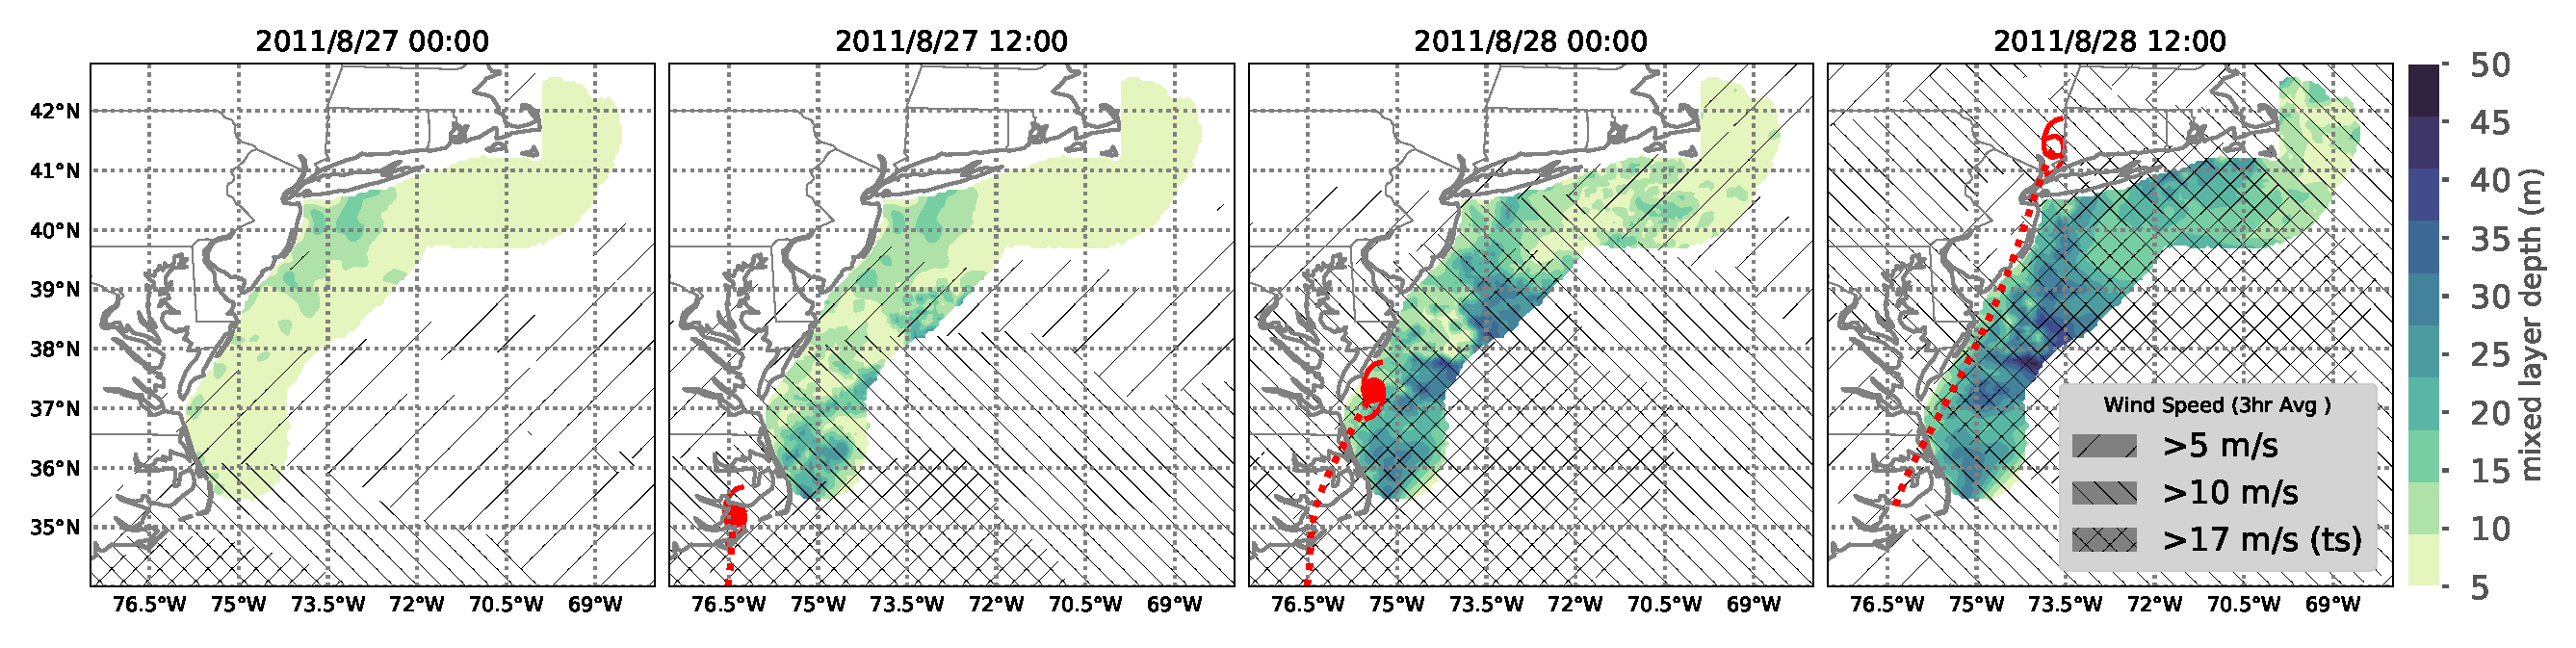
\includegraphics[width=1.0\textwidth, keepaspectratio]{irene_4panel.eps}
\end{figure}
Having the ability to remotely observe and parse the essential ocean variables involved in the mixing and entrainment of cooler water to the surface from the ahead-of-eye winds where the conditions of tropical cyclones inhibit more traditional forms of measurement, allows for nuanced and physically correct understanding of the role of the coastal ocean in controlling near-shore intensity.


Using the PMMLD algorithm we can observe the entire life cycle of the mixed layer before, during, and recovering after Hurricane Irene (Fig. 3). 
A key thing to note is that from stable MAB-wide stratification before the storm on 8/26 12:00PM to equivalently stable conditions post storm on 9/4 12:00PM requires only little more than a week despite the large wind and thermal forcing of Hurricane Irene.
\begin{figure}[h]
\caption{The full life cycle of a late-Summer/early-Fall mixed layer in response to tropical storm forcing reveals that the shallow stratification returns across the region within a week of the event, despite a much lower sea surface temperature}
\centering
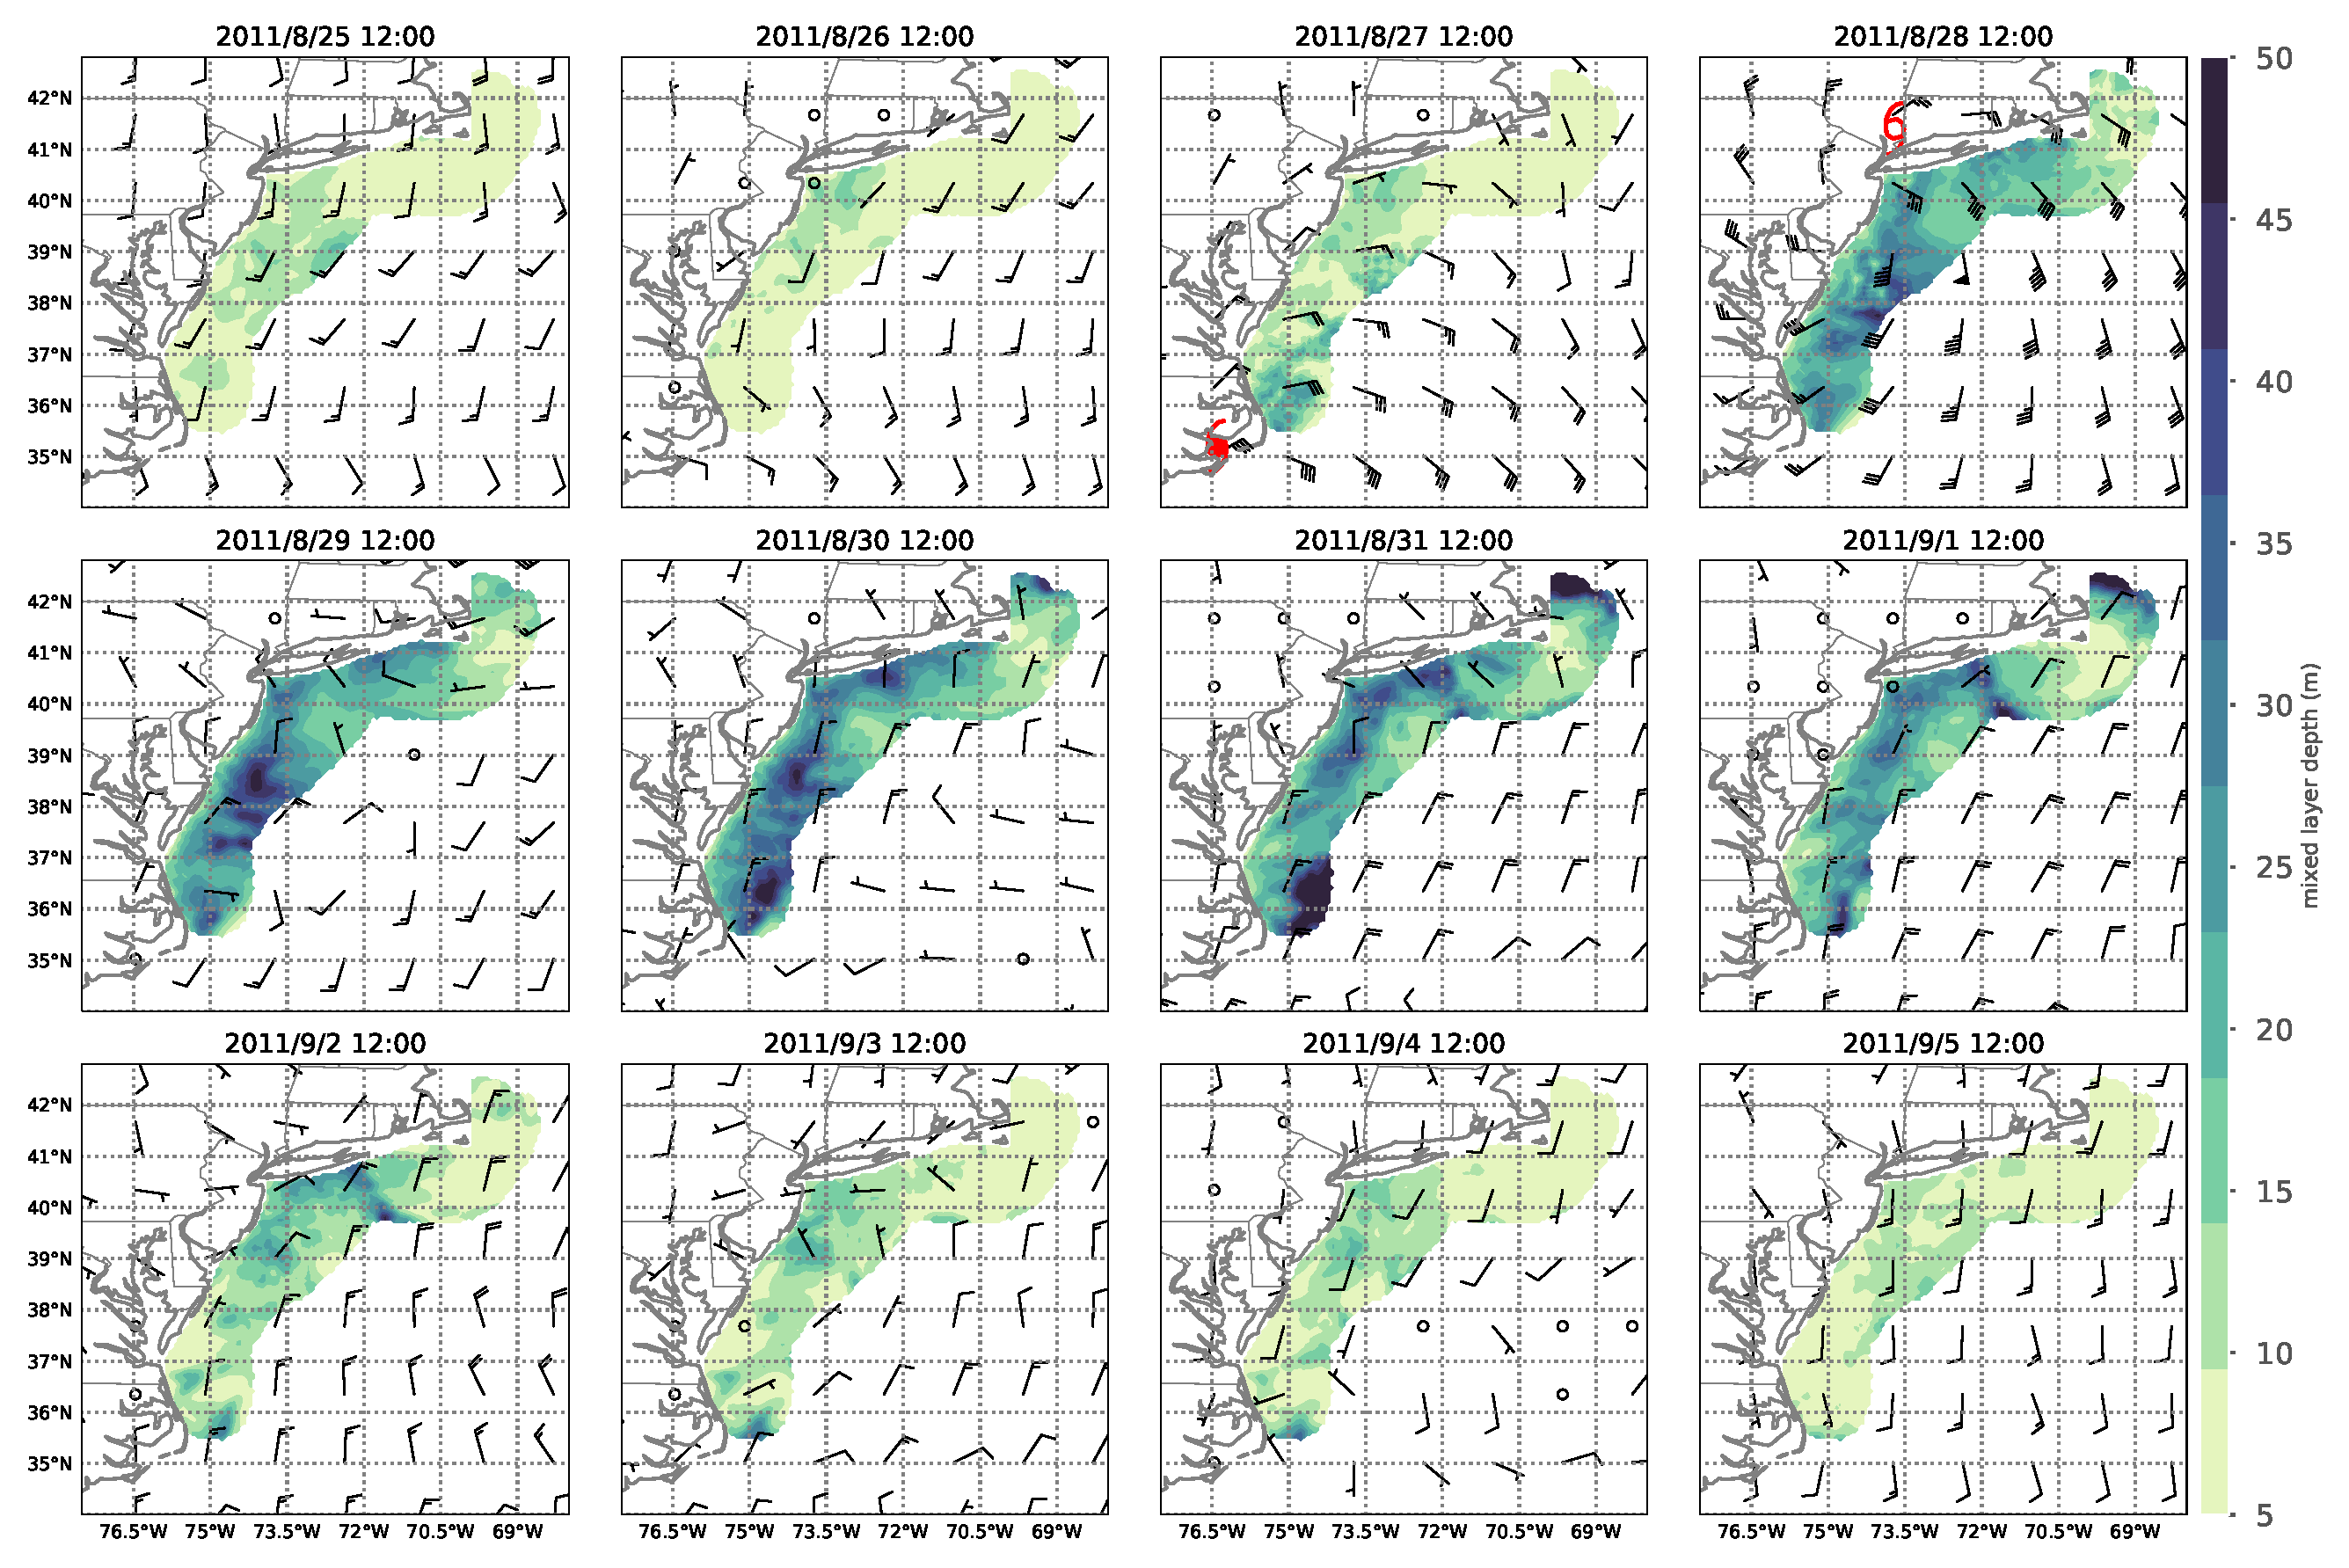
\includegraphics[width=1.0\textwidth, keepaspectratio]{irene_barbs_4koma.eps}
\end{figure}


\section*{Discussion}
The requirement of in-situ density or temperature profiles to determine the MLD severely limits our mixed-layer estimates to available CTD profiles globally, and especially in coastal oceans where changes in the MLD occur rapidly and are the leading order causal behavior for biological \cite{walsh1988simulation,fernandez1996coupling,shroyer2014stratification} and atmospheric interactions \cite{Miles2013,Seroka2016}.
By remotely observing the MLD, we can illuminate the dominant physical parameters and understand the physical processes of stratification in the MAB.
Primary production in the MAB is sustained by nutrients which originate from the off shelf waters that enter through the NE channel in the gulf of Maine and between Brownes Bank and the eastern Scotian shelf dominated by two periods of high productivity in the Spring and Fall, concurrent with changes in the MLD \cite{bigelow1933studies,marra1990phytoplankton,friedland2015spring}.
In the Summer a subsurface chlorophyll layer develops near or in the cold pool in thin layers at the pycnocline and with the onset of winter cooling and storms eroding the seasonal thermocline during October-November the subsurface summer population is replaced by a surface mixed layer population \cite{flagg1994interaction}.
Wind stress, both in average and during storm events, plays an important role in the biological timing through the development of stratification and destratification via both turbulent mixing and shelf-wide circulation \cite{Austin2002,xu2013role}.
\begin{figure}[h]
\caption{The seasonal signal of a shallow Summer mixed layer, which is strongly stratified. This shows how the dynamic transition from a uniform system to a two-layer, stratified system as the solar input changes with the season, then mixes back to a single-layer system with storm events and a decreasing solar flux.}
\centering
\includegraphics[width=1.0\textwidth, keepaspectratio]{predicted_ML_MAB_shallowing.pdf}
\end{figure}
In Figure 3, we use the PMMLD algorithm to estimate the MLD along the 50m isobath in the MAB in 2011 to show the seasonal trends.
From the Chesapeake to the Hudson Canyon shows a similar pattern dominated by the shallow (~10m) Summer MLD, indicating a robust dynamical cold pool that controls biological and physical responses. 
However, we see a markedly different pattern off the coast of Martha's Vineyard inshore of the Pioneer array, where the MLD is modulated by the cross-slope exchange \cite{gawarkiewicz2018changing}.
The Winter to Spring transition in the MAB shows a slight temporal trend starting from South moving rapidly northward, indicating the importance of solar radiation but further study is required to statistically validate the transition and develop a climatology by estimating multiple years.

\section*{Conclusion}
In this paper, we show the capability and value of using HF-radar to remotely sense the oceanic mixed layer depth.
The mixed layer represents the interface of the ocean with the atmosphere and with the sun-drenched surface ocean with the nutrients held deeper \cite{taylor2011ocean}. 
In 1970 Pollard and Millard proposed a simple two-layer slab model of for the inertial response of the mixed layer to wind forcing \cite{Pollard1970a,Pollard1970}. 
Using HF-radar to measure the near-inertial currents and North American Regional Reanalysis 10-meter winds, we developed the Pollard-Millard Mixed Layer Depth (PMMLD) as an inverse problem to find the MLD, where the slab response most closely matched the observed ocean.
Then using the abundance of autonomous underwater vehicles in the region, we tuned the model parameters to minimize the error between \textit{in situ} and predicted MLDs. 

The goal of this research was to understand both the synoptic and the seasonal trends in MLD in the MAB. 
By remotely sensing the MLD with HF-radar, we were able to get near-continuous and spatially coherent data over the entire shelf. 
As a pertinent example, we show the rapid deepening of the MLD before eye-passage of Hurricane Irene, matching previous studies and illuminating the role of mixing in the rapid de-intensification of the tropical cyclone \cite{Seroka2016}.
In addition to the information already known from \textit{in situ} AUVs, we also able to show how the changes in MLD progressed from South to North along with the storm and rebounded after the storm passed within a week.
The rapid, shelf-wide behavior of the mixed layer reveals previously unseen elements of restratification and further how the MLD behaves over the entire region during the fall breakdown of the MAB cold pool.
Using the PMMLD model, we also investigated the development and breakdown of seasonal stratification along the MAB.
More studies looking using sea surface temperature to characterize the surface heat content along with the spatial map of mixed layer can be used to show the process of heat loss of heat loss during the Autunm and in the influence of storms versus solar input in the seasonal transition of the MAB. 



\newpage
\singlespacing
\printbibliography


 
\end{document}